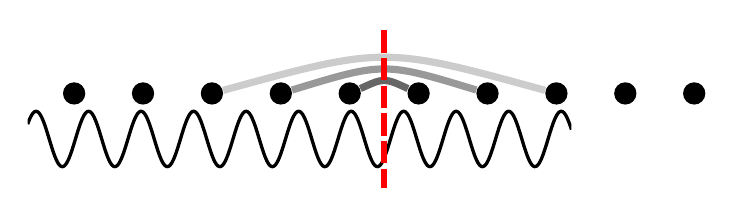
\begin{tikzpicture}[inner sep=1mm]


\begin{axis}[
	  width=0.7\textwidth,
      height=0.2\textwidth,
      axis x line=none,
      axis y line=none,
      domain=-0.5:31.91592,
      samples=501,
      xmin=-0.5, xmax=31.91592,
  	  ymin=-0.1, ymax=1.1
    ]
    \addplot [very thick] {cos(57.5*x)*cos(57.5*x)};
\end{axis}

\foreach \i in  {1,...,10} {
	\node[circle,radius=0.1,fill=black] (p\i) at (0.875*\i -0.285,1) {};
	%\filldraw[radius=0.1,fill=black] (0.875*\i -0.285,0.75) circle;
};


\draw[-,line width=2.6pt,color=black,opacity=0.6] (p5) .. controls (0.875*5.5 -0.285, 1.2) .. (p6);
\draw[-,line width=2.6pt,color=black,opacity=0.4] (p4) .. controls (0.875*5.5 -0.285, 1.4) .. (p7);
\draw[-,line width=2.6pt,color=black,opacity=0.2] (p3) .. controls (0.875*5.5 -0.285, 1.6) .. (p8);

\draw[red, dashed, line width=2pt,dash pattern=on 8pt off 2pt] (0.875*5.5 -0.285,1.8) -- (0.875*5.5 -0.285,-0.2);

\end{tikzpicture}